\chapter{Vervolg}
\label{ch:vervolg}

In dit hoofdstuk zullen mogelijke vervolgen en toepassingen van deze bachelorproef beschreven worden. Hoe kunnen anderen toegang krijgen tot de programmeercode, de website raadplegen of hoe kan de \textit{webserver} geïnstalleerd worden binnen het HOGENT-netwerk. Ook zal er besproken worden hoe de data beter en objectiever gelabeld kan worden. Omdat het doelpubliek van dit hoofdstuk anders is dan het doelpubliek van het meer technische luik van dit onderzoek, zal alles zo eenvoudig mogelijk uitgelegd worden.

\section{Applicatie-code delen}
Om er zeker van te zijn dat deze bachelorproef niet onder het stof verdwijnt en de applicatie niet meer gebruikt zal worden, is het noodzakelijk dat de volledige programmacode gedeeld kan worden. Hiervoor zal ``GitHub'' gebruikt worden.

Om het principe van GitHub te begrijpen, is het eerst nodig te verstaan wat Git zelf is. Git is een open source versiebeheersysteem. Telkens ontwikkelaars met de eigen code aan de slag gaan en hun eigen wijzigingen aanbrengen, worden op die manier de verschillen in code opgeslagen. Versiebeheersystemen beheren deze revisies door alle wijzigingen op te slaan in een centrale opslagplaats. Hierdoor kunnen ontwikkelaars gemakkelijk samenwerken, omdat ze een nieuwe versie van de software kunnen downloaden, wijzigen en zelf nieuwe revisies kunnen uploaden. Elke programmeur van dat project kan dan op zijn of haar beurt opnieuw zien welke wijzigingen er doorgevoerd zijn en kan deze opnieuw downloaden~\autocite{Brown2019}.

GitHub is dus zo een voorbeeld van een centrale opslagplaats waar alle wijzigingen opgeslagen zijn in de \textit{cloud}.

Alle code, bestanden en revisies van deze volledige bachelorproef zijn dan ook te vinden op de persoonlijke GitHub-link: \url{https://github.com/SibianDG/BachelorProef}. Wanneer iemand toegang wil, dan kan die een e-mail sturen naar Jorrit Campens die u dan in contact brengt met de schrijver, Sibian De Gussem.

De code zal ook bijgevoegd worden op de scriptietool van HOGENT als bijlage, maar er kan niet gegarandeerd worden dat dit de recentste code is.

\section{Hosting en bereikbaarheid van de applicatie}
Om te kunnen bespreken hoe men de applicatie het best beschikbaar maakt, is het nodig om de theoretische achtergrond van hosting te vermelden.

De huidige opstelling van dit eindwerk is geïllustreerd in figuur~\ref{fig:opstelling_bachelorproef}. Daarbij is alle code geïnstalleerd, op die lokale computer. Wanneer het bestand `website.py' wordt uitgevoerd, zal Python de code uitvoeren en een webserver opzetten op die lokale machine. In de output verschijnt er dan een website adres, langs waar de applicatie gebruikt kan worden.

\begin{figure}
    \centering
    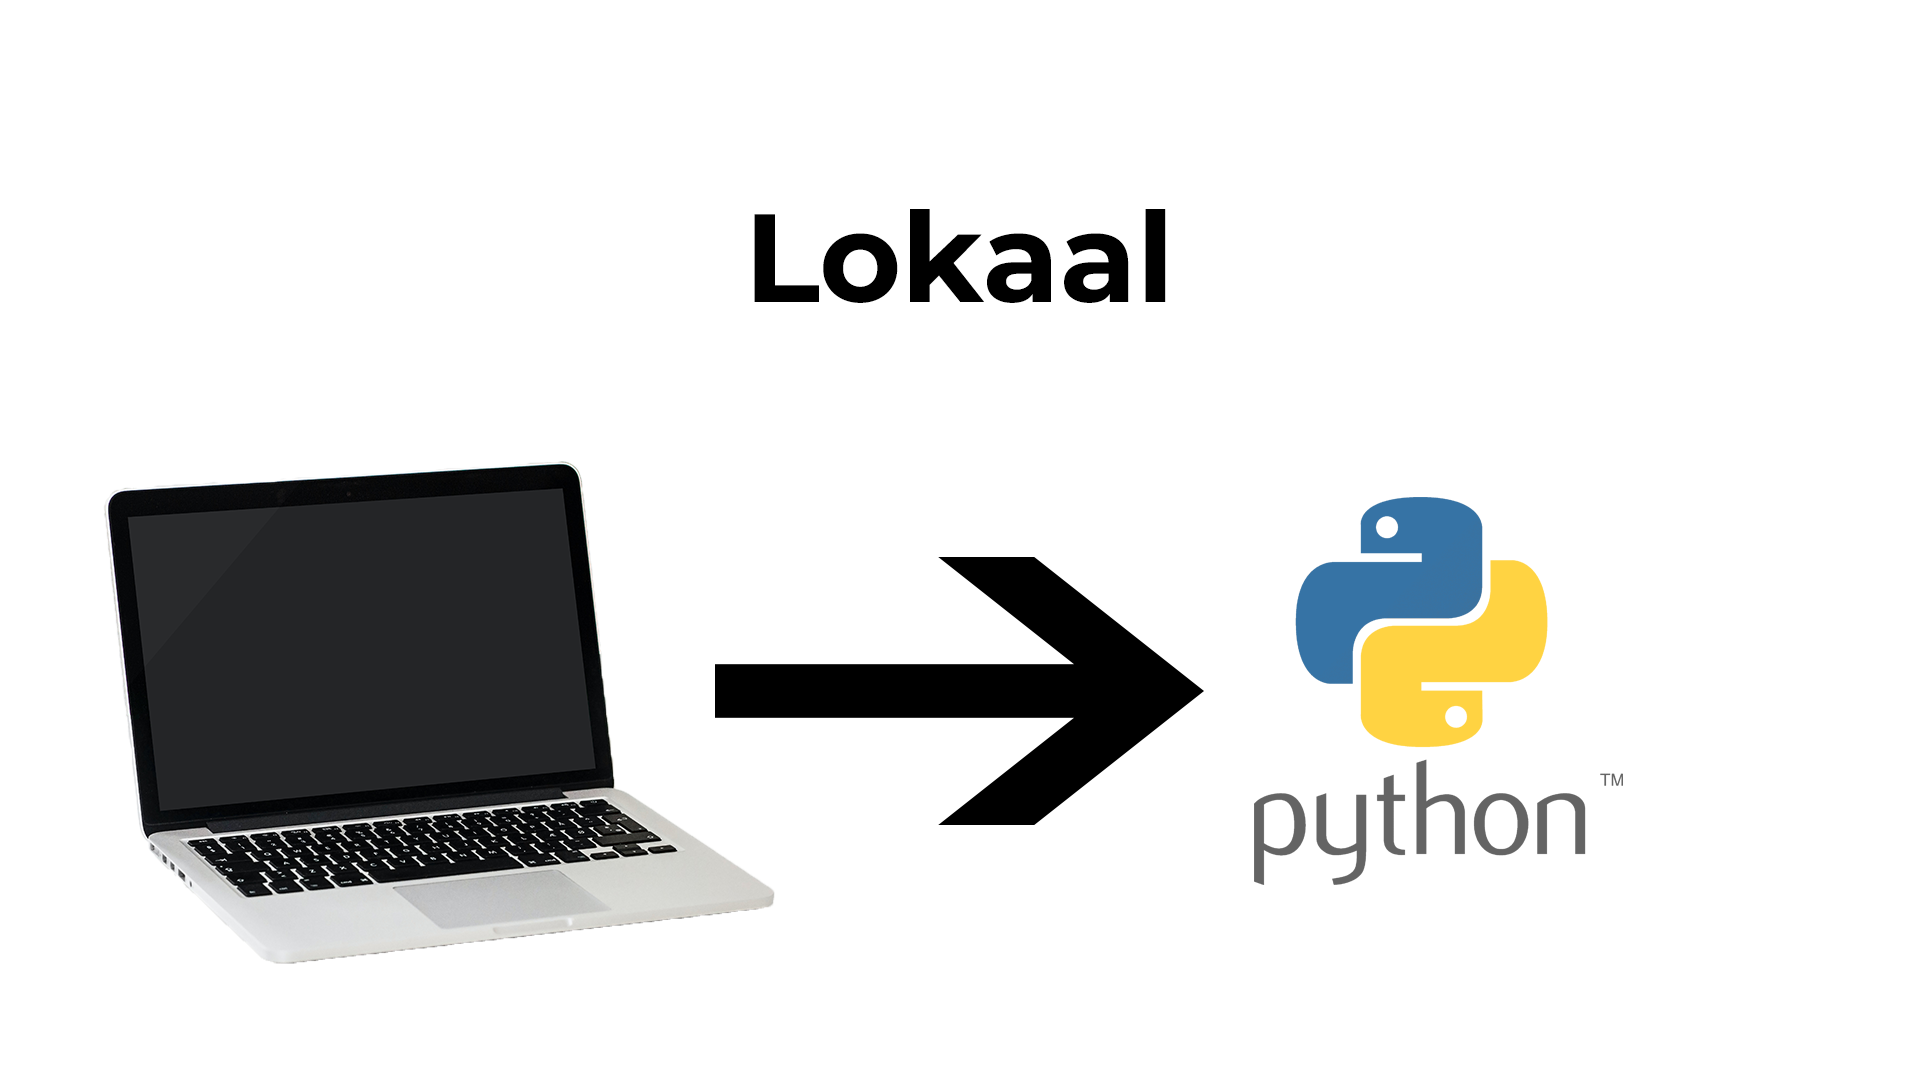
\includegraphics[width=0.75\textwidth]{./img/lokaal_website}
    \caption{\label{fig:opstelling_bachelorproef} Opstelling bachelorproef}
\end{figure}

Wanneer de website beschikbaar gemaakt moet worden voor meerdere computers moet de code op een server geïnstalleerd worden, maar een server kan ook een gewone computer zijn. Zo kunnen er meerde \textit{clients} een aanvraag of \textit{request} sturen naar de server. Die zal alles verder afhandelen, waaronder het tonen van de webpagina en het uitvoeren van de berekeningen. Een illustratie is te vinden in figuur~\ref{fig:webhosting_scheme}. Daarbij is te zien dat een verzoek verstuurd wordt naar het internet wanneer een gebruiker of \textit{user} naar een website surft. Het internet weet op zijn beurt aan welke webserver het informatie kan vragen of sturen.
De rol van de server is het afhandelen van de html-, en JavaScript-pagina's, websitebestanden, en doet ook de berekeningen.

\begin{figure}
    \centering
    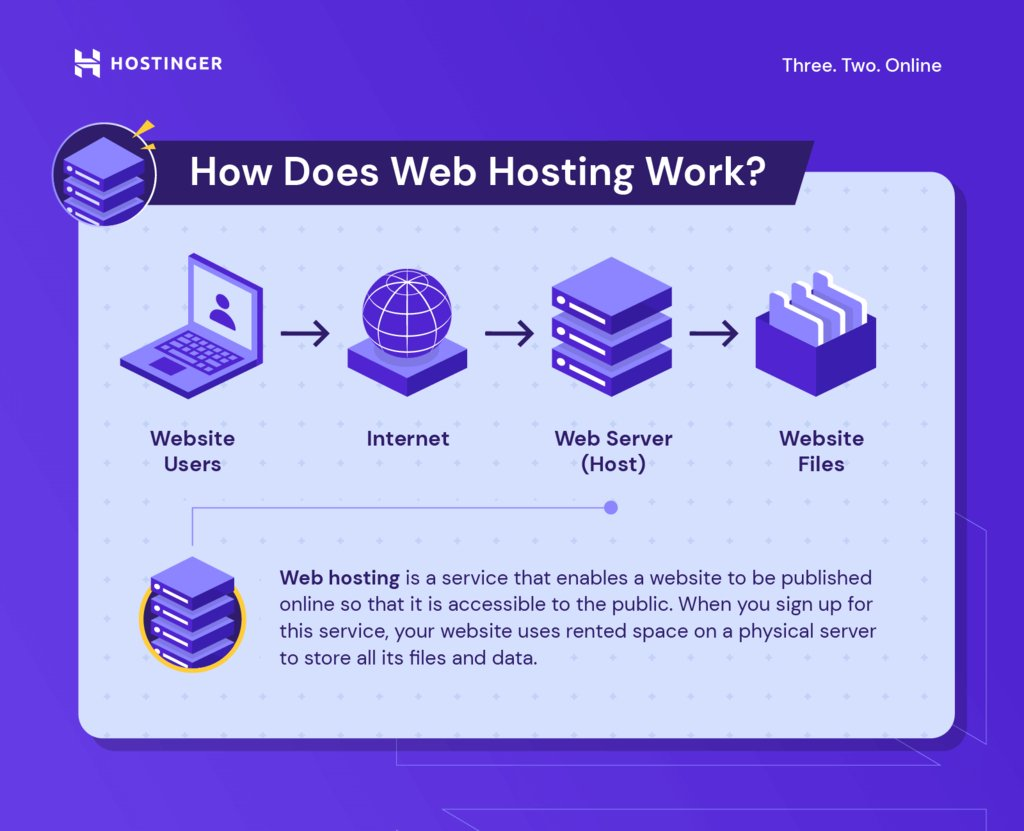
\includegraphics[width=0.8\textwidth]{./img/how-does-web-hosting-work}
    \caption{\label{fig:webhosting_scheme} Hoe werkt webhosting~\autocite{Tamara2022}.}
\end{figure}

\subsection{Installeren op een computer}
In de hoofdmap met alle code is er een bestand te vinden genaamd ``requirements.txt''. Door het commando:
\begin{python}
    pip install -r requirements.txt
\end{python}
uit te voeren zullen alle Python-bibliotheken geïnstalleerd worden die nodig zijn om het project uit te voeren. Er dient wel nog een extra stap gebeuren, namelijk FFmpeg apart installeren. De instructies daarvan staan beschreven op de volgende website: \url{https://www.wikihow.com/Install-FFmpeg-on-Windows} voor een Windows besturingssysteem.

\subsubsection{Voordelen}
\begin{itemize}
    \item Snelle opzet voor IT'ers.
    \item Snelle verwerking, omdat het op één computer gebeurt en er maar één persoon toegang heeft.
    \item Gratis oplossing.
\end{itemize}
\subsubsection{Beperkingen}
\begin{itemize}
    \item Andere computers hebben geen toegang
    \item Niet-IT'ers kunnen het mogelijk minder makkelijk installeren
    \item De software zou op elke computer opnieuw geïnstalleerd moeten worden.
\end{itemize}

\subsection{Hosten in een lokaal netwerk}
Het is ook mogelijk om de software op een computer te installeren, met een speciale parameter. Wanneer in de Flask-applicatie de volgende parameter `` host=`0.0.0.0' '' wordt meegegeven, zal de applicatie opengesteld worden in het lokale netwerk. Dit maakt het mogelijk om naar het lokale IP-adres te surfen met een ander toestel en ook de website met de detector te gebruiken. Als men het argument \textit{threaded} op \textit{true} zet, dan is Flask \textit{multithreaded}~\autocite{Vieira2013}. Hierdoor kunnen er zeker meerdere toestellen tegelijk verbonden worden. Een systematische voorstelling is te vinden in figuur~\ref{fig:lokaal_netwerk}. Wanneer men verbonden is met het Eduroam-netwerk, het netwerk dat in elke hogeschool of universiteit aanwezig is, dan zal dit niet lukken volgens de IT-dienst van HOGENT: ``Binnen het Eduroam-netwerk is het niet mogelijk dat andere toestellen aan jouw eigen toestel kunnen.''.

\subsubsection{Voordelen}
\begin{itemize}
    \item Een eenmalige installatie op een computer, bijvoorbeeld de docent, is voldoende om het programma altijd te kunnen opstarten in de les.
    \item Meerdere connecties zijn mogelijk.
    \item Het is een gratis oplossing
\end{itemize}
\subsubsection{Beperkingen}
\begin{itemize}
    \item Het maximale aantal connecties is afhankelijk van de computer waarop de applicatie wordt opgestart. Hoe beter en sneller de computer is, hoe meer connecties mogelijk zijn en hoe sneller de applicatie functioneert.
    \item Er moet een SSL-certificaat gemaakt en geïnstalleerd worden voor een beveiligde HTTPS-verbinding.
    \item Het is niet mogelijk op het Eduroam-netwerk.
\end{itemize}

\begin{figure}
    \centering
    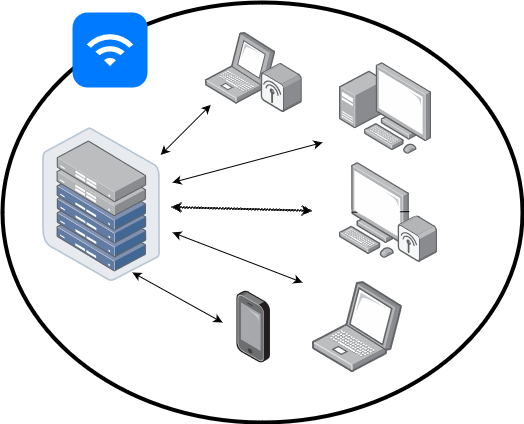
\includegraphics[width=0.75\textwidth]{./img/lokaal_netwerk}
    \caption{\label{fig:lokaal_netwerk} Lokaal netwerk}
\end{figure}

\subsection{Hosting online}
De applicatie kan ook online gehost worden, maar dit zal natuurlijk geld kosten. Zo'n applicatie kan dan gehost worden op Microsoft Azure als webapplicatie, maar ook via Combell. Elke student en docent krijgt zo driejaarlijks een website op de volgende link: \url{https://www.academicsoftware.eu/software/298/857}.
\subsubsection{Mogelijkheden}
\begin{itemize}
    \item Eens opgezet is het altijd en overal beschikbaar.
    \item Wanneer er veel verbindingen en berekeningen nodig zijn, zullen de servers van de aanbieder automatisch geüpgraded worden zodat ze alles kunnen bolwerken.
    \item Heel snelle bewerkingen.
\end{itemize}
\subsubsection{Beperkingen}
\begin{itemize}
    \item Dit zorgt voor een grote financiële kost.
\end{itemize}

\subsubsection{Hosten via Docker}
Een mogelijkheid is ook om de website te hosten via ``Docker''. Docker is een container-technologie waar in één container draait. Maar deze optie lag buiten de scope van dit eindwerk. Toch kan dit eventueel dienen als vervolg voor de richting toegepaste informatica: ``Host de \textit{elderspeak}-website met een Docker-container.''.

\section{Testen}
Het aantal testen dat verzameld werd, is niet van een bijzonder grote grootteorde. Er kunnen extra testen, in de vorm van nieuwe audio-opnames, opgenomen worden in een vervolgopdracht. Dit kan een interdisciplinaire opdracht zijn met de richting verpleegkunde, communicatie en eventueel toegepaste informatica. Immers hoe meer testen, hoe groter de accuraatheid van de applicatie.

Een mogelijke opzet van deze opdracht wordt hier besproken. De studenten verpleegkunde maken en/of klasseren audio-opnames van eventuele \textit{elderspeak}.

Studenten uit communicatierichtingen kunnen alle data dan opnieuw labelen, aangezien zij veel kennis hebben rond dit fenomeen. Zo kan de data zeer nauwkeurig en uitgebreid geanalyseerd worden, terwijl in dit eindwerk de data gelabeld werd door een persoon die geen expert is.

Toch kunnen de studenten informatica ook betrokken worden. Ze kunnen zelf een programma schrijven om de gelabelde data te laten analyseren door de applicatie. Dit is evenwel al beschikbaar in de bachelorproef, maar beginnende studenten kunnen door deze opdracht gestimuleerd worden met een goed voorbeeld en een duidelijk doel. Wanneer de data uitgebreider geanalyseerd wordt, moeten de testen enigszins herschreven worden, wat ook een oefening kan zijn.
